\documentclass[11pt]{article}
\usepackage[margin=1in]{geometry}
\usepackage{graphicx}
\usepackage{amsmath,amssymb}
\usepackage{booktabs}
\usepackage{hyperref}
\usepackage{listings}
\usepackage{xcolor}
\usepackage{float}

\lstset{
  basicstyle=\ttfamily\small,
  keywordstyle=\color{blue},
  commentstyle=\color{gray},
  breaklines=true,
  frame=single
}

\title{Optimal Light Spectra Under Regulatory Constraints:\\
       How Efficiency Standards Drive Lamps to Weird Spectral States}
\author{Generated by \texttt{photopic} --- a Modula-3/Scheme spectral optimizer}
\date{March 2026}

\begin{document}
\maketitle

\begin{abstract}
Government regulations on lamp efficiency (lumens per watt) and color quality
(Color Rendering Index) define a constrained optimization problem whose
solutions are not the smooth, broad spectra of incandescent bulbs but
narrow-band, spiky spectral power distributions.  We use \texttt{photopic},
a hybrid Modula-3/Scheme numerical tool, to explore the Pareto frontier of
this trade-off.  As the efficacy requirement increases, the optimal spectrum
converges to approximately three narrow peaks near 450, 540, and 610~nm ---
Thornton's ``prime color'' wavelengths --- while aggressively suppressing
power at all other wavelengths, including the red region critical for color
fidelity.  The results show that regulatory pressure, when pushed to its
logical extreme, drives light sources toward spectra that are visually
``weird'': they satisfy the letter of color rendering standards while
producing light that many people find unnatural.
\end{abstract}

\section{Introduction}

An incandescent lamp is a near-perfect blackbody radiator.  Its spectrum is
broad and smooth, rendering colors with perfect fidelity (CRI~$=$~100).
But most of its radiation falls in the infrared, giving it a luminous efficacy
of only $\sim$15~lm/W.  Government regulations worldwide --- EU Ecodesign,
US EISA/DOE, California Title~24 --- have mandated minimum efficacy standards
that incandescent lamps cannot meet, effectively banning them.

The replacement technologies (fluorescent, LED) achieve high efficacy by
concentrating their emission in the visible spectrum.  But \emph{where} in
the visible spectrum?  The CIE photopic luminous efficiency function $V(\lambda)$
peaks sharply at 555~nm (yellow-green).  A monochromatic source at 555~nm
would achieve the theoretical maximum of 683~lm/W --- but it would render
no colors at all.

The question becomes: \textbf{What spectral power distribution maximizes
luminous efficacy while maintaining acceptable color rendering?}

This is a constrained optimization problem.  The constraints come from
regulations:
\begin{itemize}
\item \textbf{CRI $\geq$ 80} (Energy Star, EU); CRI $\geq$ 90 (California Title~24 for some applications)
\item \textbf{CCT within $\pm$50K} of the nominal color temperature (e.g., 2700K for ``warm white'')
\item \textbf{Duv $\leq$ 0.012}: chromaticity tolerance (distance from the blackbody locus)
\end{itemize}

We explore what happens as you ``turn up the knob'' on the efficacy
requirement.  The answer is surprising: the optimal spectra become
increasingly bizarre.

\section{Background}

\subsection{Luminous Efficacy}

Luminous efficacy of radiation (LER) is the ratio of luminous flux to radiant
power:
\begin{equation}
\eta = K_m \frac{\int_0^\infty S(\lambda)\, V(\lambda)\, d\lambda}
                {\int_0^\infty S(\lambda)\, d\lambda}
\end{equation}
where $S(\lambda)$ is the spectral power distribution, $V(\lambda)$ is the
CIE 1931 photopic luminous efficiency function, and $K_m = 683$~lm/W is the
maximum luminous efficacy at 555~nm.

For a 2700K blackbody, the total LER is only $\sim$15~lm/W because most
radiation is in the infrared.  If we restrict to the visible band
(380--770~nm), the visible-only LER is $\sim$88~lm/W.

\subsection{Color Rendering Index (CRI)}

The CRI quantifies how faithfully a light source renders colors compared to a
reference illuminant (a blackbody at the same correlated color temperature).
The calculation, following CIE 13.3-1995 and the colorimetric formulas in
Foley and van~Dam~\cite{foley-vandam}, involves:

\begin{enumerate}
\item Normalize the test spectrum to $Y=100$
\item Find the reference blackbody at the correlated color temperature (CCT)
      via search in CIE~1960 MacAdam $(u,v)$ space
\item For each of 14 Test Color Samples (TCS), compute the color shift
      $\Delta E^*_{UVW}$ using von~Kries chromatic adaptation
\item $R_i = 100 - 4.6\,\Delta E^*_{UVW}$ for each sample; $\text{CRI}(R_a) =
      \frac{1}{8}\sum_{i=1}^{8} R_i$
\end{enumerate}

The key subtlety: only TCS~1--8 contribute to $R_a$.  TCS~9 (saturated red)
is \emph{not} part of the official CRI score.  This creates a loophole that
the optimizer exploits.

\subsection{Thornton's Prime Colors}

In 1971, W.~A.~Thornton of Westinghouse showed that the most chromatically
effective wavelengths for white light are three narrow bands near
\textbf{450, 540, and 610~nm} --- the ``prime colors''~\cite{thornton1971}.
Conversely, wavelengths near 500~nm and 580~nm are ``anti-prime'' ---
they contribute power without adding chromaticity discrimination.
Thornton was named US National ``Inventor of the Year'' in 1979 for his
prime-color fluorescent lamp patents~\cite{thornton-inventor}.

The optimization results below independently rediscover Thornton's prime
colors from first principles.

\section{The \texttt{photopic} Tool}

\texttt{photopic} is a hybrid application: performance-critical spectral
calculations (Planck's law, CIE color matching functions, numerical
integration) are implemented in compiled Modula-3~\cite{modula3,cm3}
libraries, while the optimization driver, CRI calculation, and plotting
are written in Scheme using MScheme~\cite{mscheme}, a Scheme
interpreter embedded in the Modula-3 runtime.  MScheme's \texttt{sstubgen}
tool automatically generates Scheme bindings from Modula-3 interfaces,
allowing the Scheme code to manipulate compiled M3 objects (spectral
arrays, integration routines, color-matching data) directly without
marshalling overhead.  This architecture provides the rapid prototyping
benefits of a scripting language for the optimization logic while
retaining compiled-language performance for the inner numerical loops.

\subsection{Architecture}

\begin{center}
\begin{tabular}{ll}
\toprule
\textbf{Component} & \textbf{Role} \\
\midrule
\texttt{Blackbody.m3}          & Planck radiance $B_\nu(T,\nu)$ \\
\texttt{CieSpectrum.m3}        & Photopic $V(\lambda)$, conversion to lumens \\
\texttt{CieXyz.m3}             & CIE 1931 $\bar{x},\bar{y},\bar{z}$ color matching \\
\texttt{Tcs.m3}                & 14 Test Color Sample reflectance spectra \\
\texttt{TempUv.m3}             & Blackbody locus in $(u,v)$ for CCT search \\
\texttt{ParametricSpectrum.m3} & Piecewise-linear log-amplitude parameterization \\
\texttt{COBYLA\_M3.m3}         & Constrained optimization (Powell's COBYLA) \\
\texttt{NR4p4.m3}              & Romberg integration (midpoint rule) \\
\texttt{Bracket.m3}            & Brent's method for CCT root-finding \\
\texttt{photopic.scm}          & Optimization driver, CRI calc, plotting \\
\bottomrule
\end{tabular}
\end{center}

\subsection{Spectrum Parameterization}

The optimizer works in log-amplitude space.  A test spectrum is represented as:
\begin{equation}
S(\lambda) = \exp\!\bigl(f(\lambda)\bigr) \cdot B_\lambda(T_0, \lambda)
\end{equation}
where $B_\lambda(T_0, \lambda)$ is the baseline blackbody at the target CCT,
and $f(\lambda)$ is a piecewise-linear function defined by $n$ parameters
(control points evenly spaced across 380--770~nm).

The resolution increases through \emph{hierarchical subdivision}:
$n = 2 \to 3 \to 5 \to 9 \to 17 \to 33 \to 65 \to 129$.  At each level,
COBYLA~\cite{powell1994} minimizes the negative efficacy subject to CRI, CCT,
and chromaticity constraints.  The solution from level $n$ is interpolated
to initialize level $2n-1$.

\subsection{Objective Function}

The optimization target vector passed to COBYLA is:
\begin{equation}
\mathbf{t} = \begin{pmatrix}
-\eta \\
R_a - R_a^{\min} \\
R_9 - R_9^{\min} \\
R_{\min} - (R_a^{\min} - 10) \\
\text{CCT} - (T_0 - 50) \\
(T_0 + 50) - \text{CCT} \\
1000\,(0.012 - D_{uv})
\end{pmatrix}
\end{equation}
where $\eta$ is the LER, and the remaining components are inequality
constraints ($\geq 0$ required).

\section{Results}

\subsection{Blackbody vs.\ Optimized Spectrum}

Figure~\ref{fig:blackbody-vs-opt} shows the dramatic difference between a
2700K blackbody and the maximum-efficacy spectrum with CRI~$\geq$~60.

\begin{figure}[H]
\centering
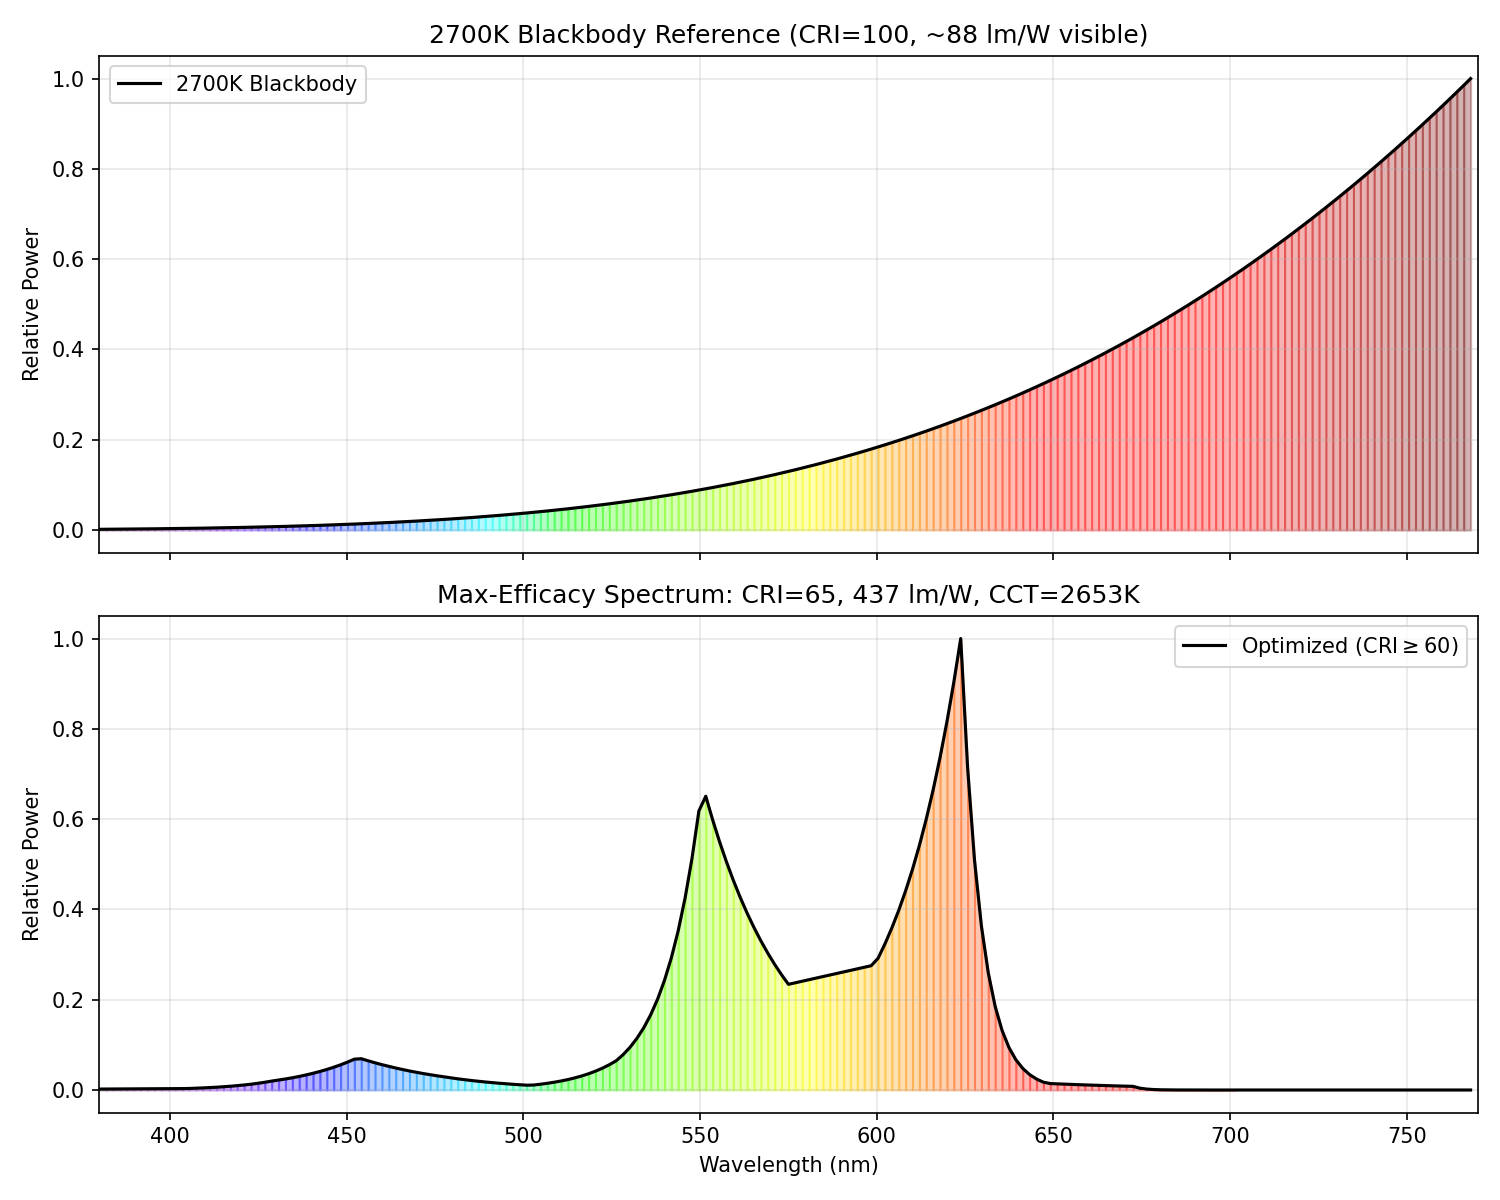
\includegraphics[width=0.85\textwidth]{fig1_blackbody_vs_optimized.png}
\caption{Top: 2700K blackbody reference spectrum (CRI~$=$~100,
  $\sim$88~lm/W visible).  Bottom: maximum-efficacy spectrum achieving
  CRI~$=$~65 at 437~lm/W.  The optimizer concentrates power into three
  peaks near Thornton's prime-color wavelengths while suppressing
  power below 500~nm and above 660~nm.}
\label{fig:blackbody-vs-opt}
\end{figure}

The optimized spectrum achieves $\sim$5$\times$ higher efficacy than the
blackbody by eliminating ``wasted'' power at wavelengths where the eye is
insensitive or where chromaticity is redundant.  The three peaks correspond
to Thornton's prime colors:
\begin{itemize}
\item \textbf{$\sim$450~nm} (blue): establishes the short-wavelength
  chromaticity anchor
\item \textbf{$\sim$540~nm} (green): near the peak of $V(\lambda)$ ---
  provides most of the lumens
\item \textbf{$\sim$610~nm} (orange-red): establishes warm color temperature
\end{itemize}

\subsection{Convergence: The Spectrum Gets ``Weirder'' with More Freedom}

Figure~\ref{fig:convergence} shows how the optimized spectrum evolves as
the number of control parameters increases from 2 to 17.

\begin{figure}[H]
\centering
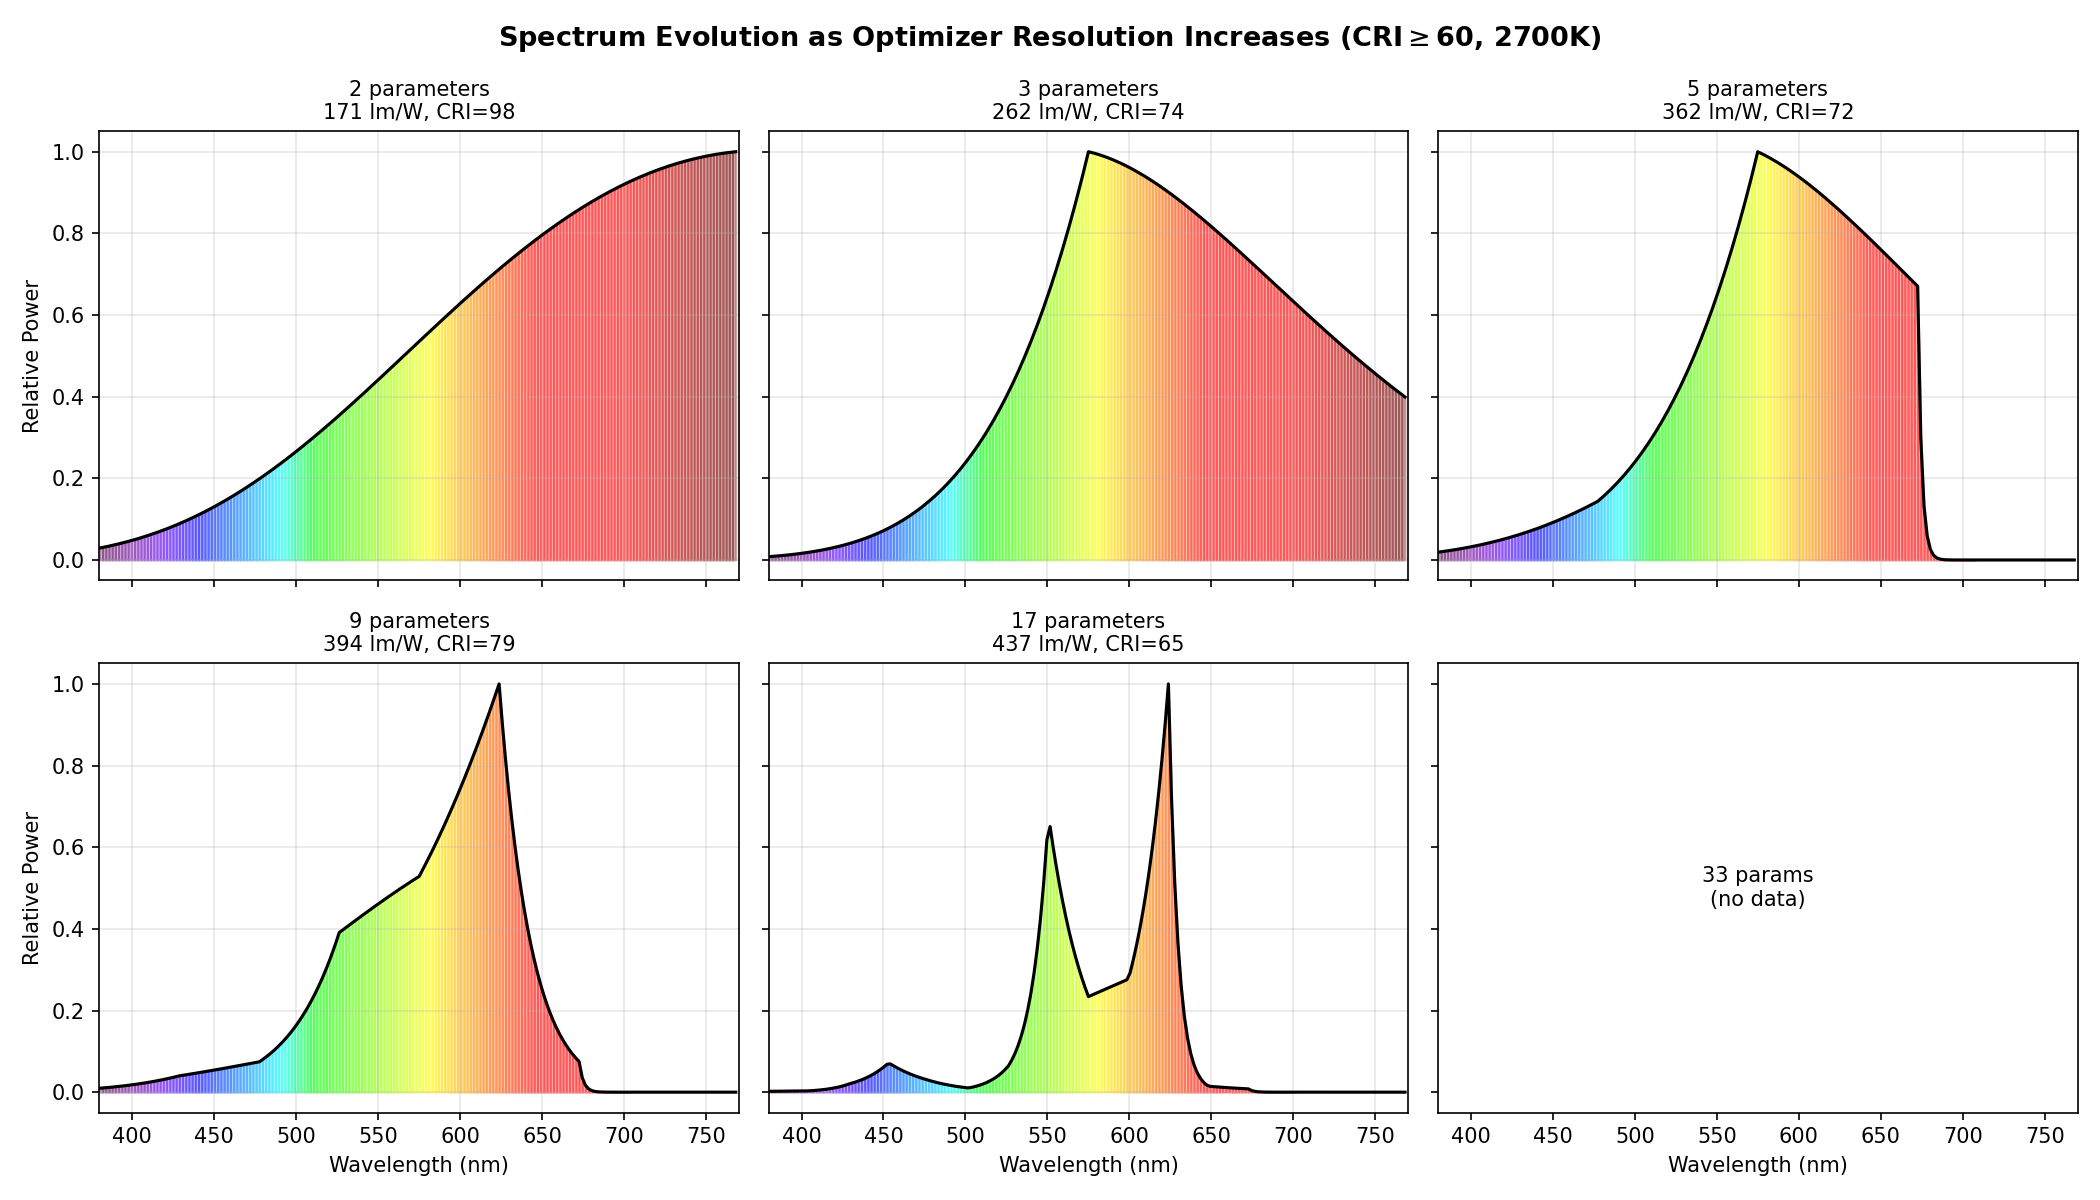
\includegraphics[width=0.95\textwidth]{fig3_convergence.png}
\caption{Evolution of the optimal CRI~$\geq$~60 spectrum at 2700K as the
  optimizer gains more spectral resolution.  With 2 parameters, the spectrum
  is nearly a tilted blackbody (171~lm/W).  As parameters increase, the
  optimizer carves out deep nulls between peaks, reaching 437~lm/W at 17
  parameters.  The three-peak structure emerges clearly by 9 parameters.}
\label{fig:convergence}
\end{figure}

The progression is illuminating:
\begin{itemize}
\item \textbf{2 parameters} (171~lm/W): Can only tilt the spectrum.  Shifts power
  toward green.  Still smooth, CRI~$=$~98.
\item \textbf{3 parameters} (262~lm/W): First sign of spectral sculpting.  Blue
  and deep red suppressed.
\item \textbf{5 parameters} (362~lm/W): Three-peak structure begins to emerge.
  Deep null around 500~nm.
\item \textbf{9 parameters} (394~lm/W): Clear three peaks with valleys between.
  CRI drops to 79.
\item \textbf{17 parameters} (437~lm/W): Fully developed spiky spectrum.
  Deep nulls, sharp peaks.  CRI just satisfies the $\geq$60 floor.
\end{itemize}

The optimizer, given enough degrees of freedom, always converges to a
three-peak solution.  \textbf{This is Thornton's prime-color theorem,
rediscovered numerically.}

\subsection{The R9 Problem}

The CRI score $R_a$ averages only TCS~1--8, which are relatively
unsaturated.  TCS~9 (saturated red) is reported separately.  When the
optimizer is free to set $R_9$ as low as $-100$, it exploits this:
the CRI~$\geq$~60 optimized spectrum at 17 parameters has $R_9 = -28$.

This means: under this ``optimal'' light, saturated reds look dramatically
wrong --- less red than under a reference illuminant.  A person wearing a
red dress would look dull; red paint would look brownish.  But the CRI
score says the light is acceptable.

This is the ``weird final state'' that regulations drive toward: a lamp
that passes the official color test while rendering an important class
of colors --- reds --- poorly.

\subsection{Effect of CRI Constraints}

Figure~\ref{fig:comparison} shows how the optimal spectrum changes as the
CRI floor increases.

\begin{figure}[H]
\centering
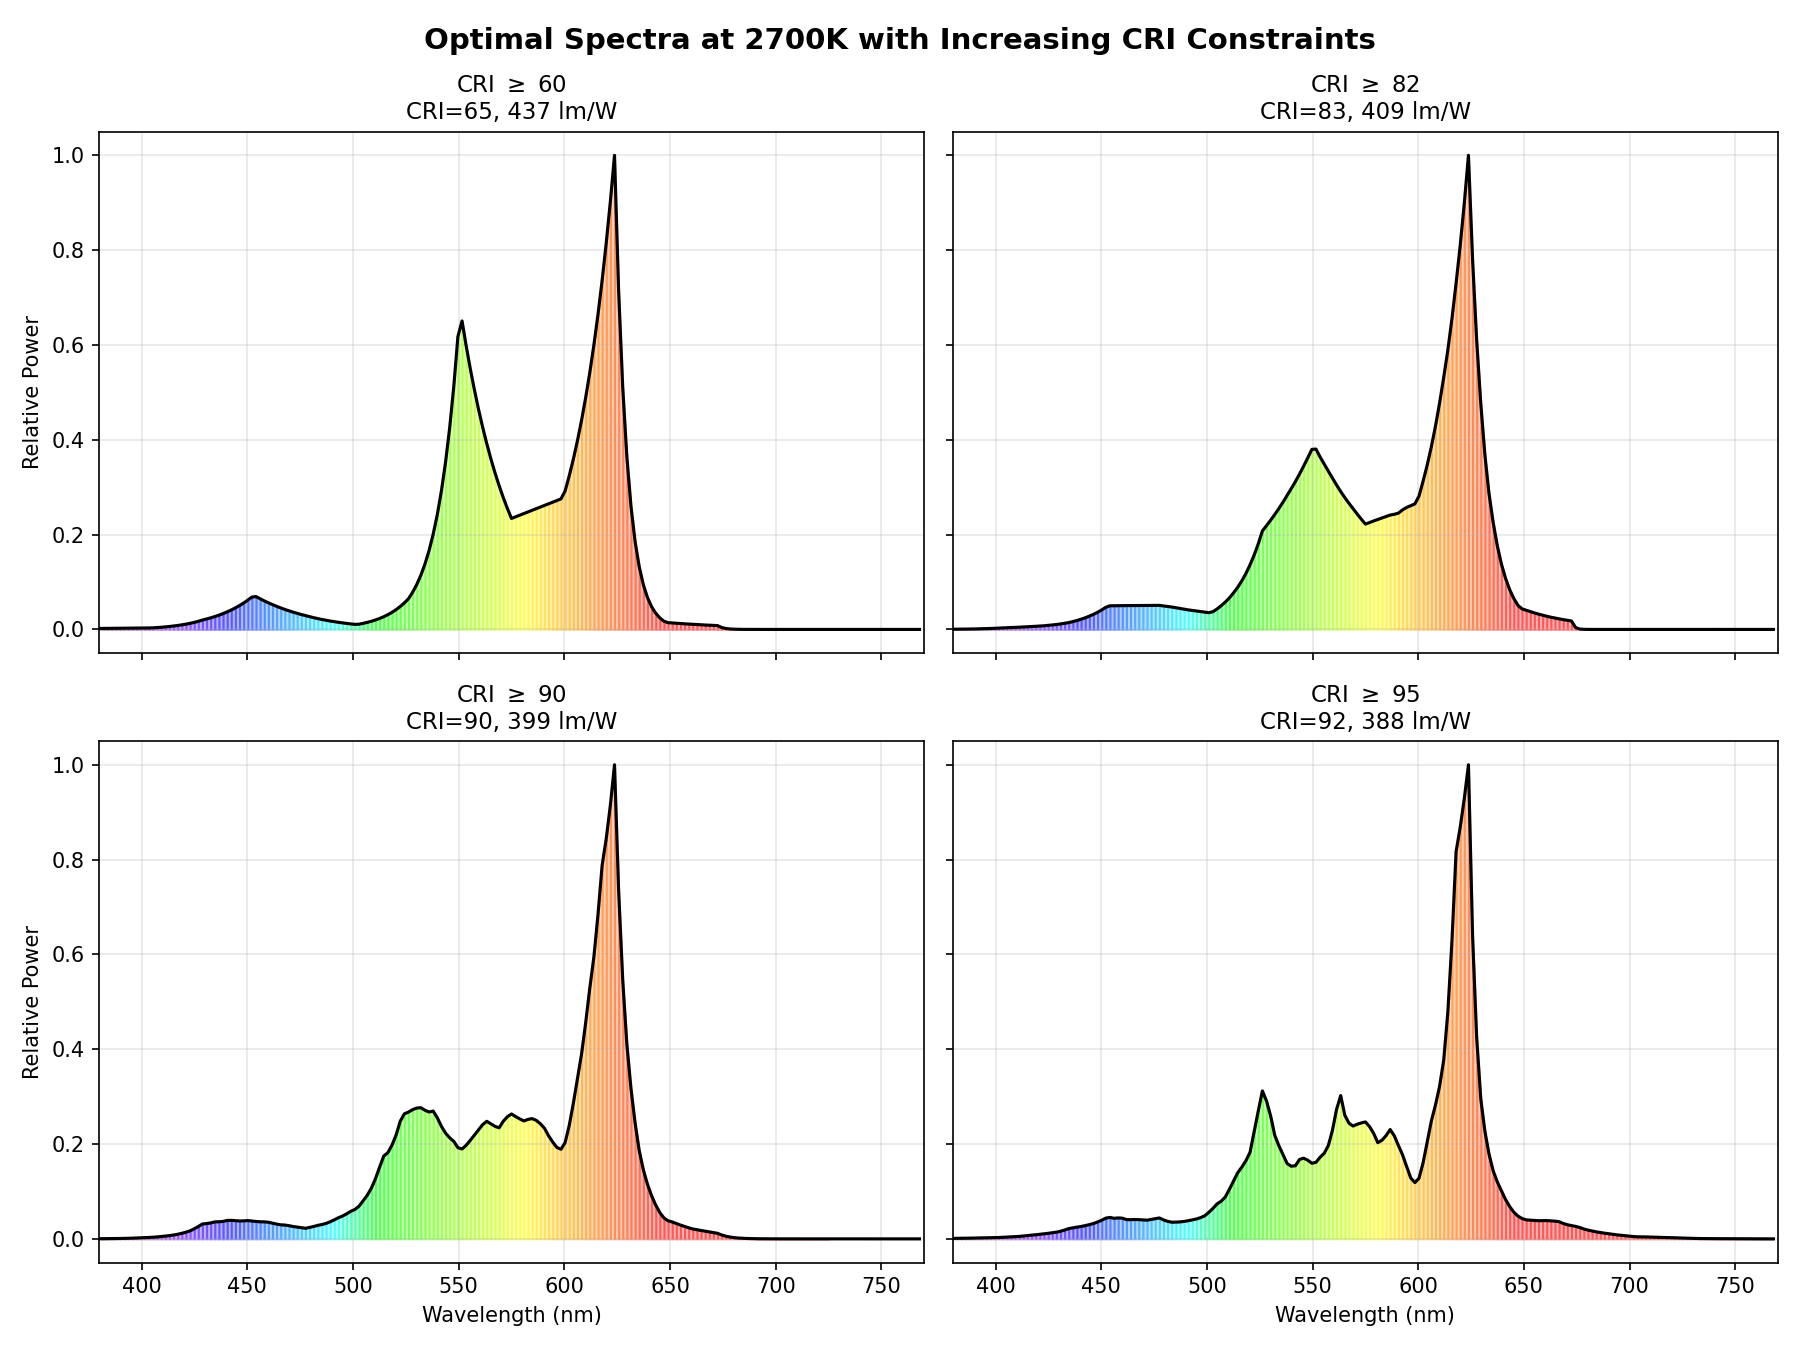
\includegraphics[width=0.85\textwidth]{fig2_cri_comparison.png}
\caption{Optimal spectra at 2700K for different CRI constraints.
  As CRI requirements increase, the spectrum must broaden to render more
  colors faithfully, reducing the maximum achievable efficacy.  The
  three-peak structure persists but the peaks must widen and the valleys
  cannot be as deep.}
\label{fig:comparison}
\end{figure}

% Table of results
\begin{table}[H]
\centering
\caption{Efficacy--CRI trade-off at 2700K CCT, unconstrained $R_9$.
  Results at 129 spectral parameters (17 for CRI~60).}
\label{tab:tradeoff}
\begin{tabular}{rrrrrl}
\toprule
Min CRI & Achieved CRI & Efficacy (lm/W) & $R_9$ & Worst $R_i$ & Character \\
\midrule
--- & 100 & 88 & 100 & 100 & 2700K blackbody (visible only) \\
60 & 65 & 437 & $-28$ & 50 & Three sharp peaks, deep valleys \\
70 & 73 & 428 & $-7$ & 60 & Three peaks, moderate valleys \\
80 & 83 & 412 & $+21$ & 70 & EU minimum: R9 still poor \\
82 & 83 & 409 & $+29$ & 72 & Three peaks, shallower valleys \\
85 & 88 & 402 & $+33$ & 75 & Transitional region \\
90 & 90 & 399 & $+45$ & 80 & Broader peaks, less suppression \\
95 & 92 & 388 & $+58$ & 86 & Wide peaks, modest valleys \\
98 & 93 & 358 & $+75$ & 89 & Approaching continuous \\
\bottomrule
\end{tabular}
\end{table}

The trade-off is dramatic: going from CRI~60 to CRI~98 costs roughly
80~lm/W of achievable efficacy (437 $\to$ 358~lm/W at 129 spectral
parameters), and the key variable is $R_9$ --- the ability to render
saturated reds.  At CRI~60, $R_9$ is deeply negative ($-28$), meaning
reds appear wrong; at CRI~98, $R_9 = 75$ and red rendering is
acceptable.

The EU regulatory minimum --- CRI~$\geq$~80 at $\sim$412~lm/W ---
achieves high efficiency but with $R_9 = 21$, meaning reds are rendered
at barely one-fifth of reference fidelity.  This is the ``weird final
state'' that market and regulatory forces converge on.  California's
JA8 standard, which requires $R_9 \geq 50$, pushes manufacturers above
CRI~90, where the achievable efficacy drops to $\sim$399~lm/W but red
rendering reaches $R_9 = 45$.

\subsection{The Pareto Frontier: Overlay of All Solutions}

Figure~\ref{fig:overlay} overlays all optimized spectra on a single plot,
together with the blackbody reference.

\begin{figure}[H]
\centering
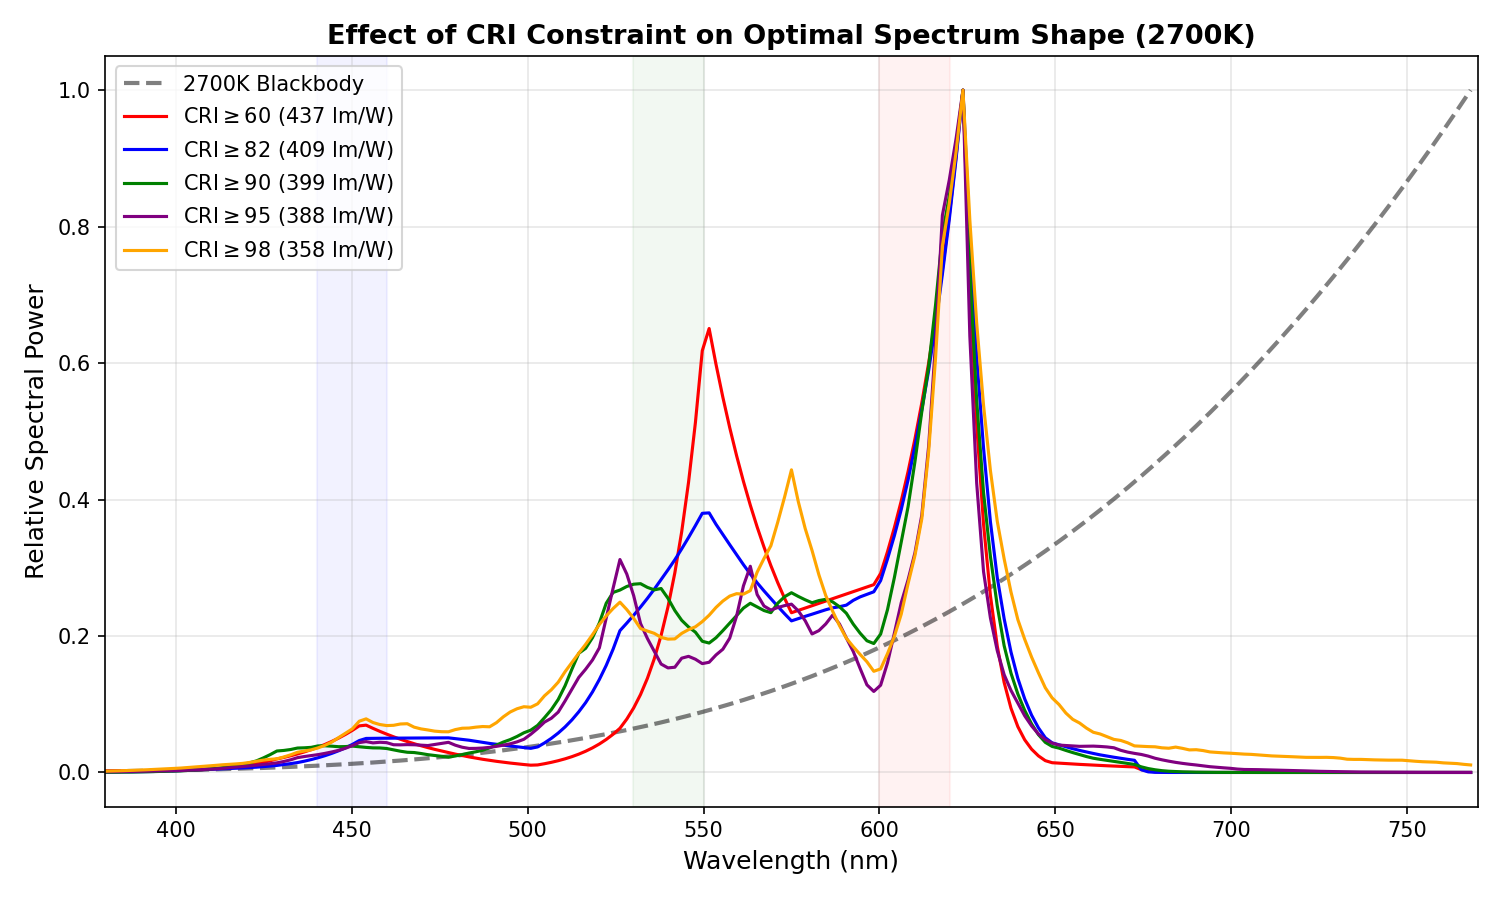
\includegraphics[width=0.85\textwidth]{fig4_overlay.png}
\caption{Overlay of optimal spectra at 2700K for CRI constraints from 60 to 98.
  All spectra share the same three-peak topology (blue $\sim$450~nm,
  green $\sim$540~nm, red $\sim$610~nm) but differ in peak width and
  valley depth.  The dashed curve is the 2700K blackbody.
  The shaded bands mark Thornton's prime-color wavelength regions.}
\label{fig:overlay}
\end{figure}

\subsection{The Efficacy--CRI Trade-off Curve}

Figure~\ref{fig:tradeoff} plots the maximum achievable efficacy as a function
of the CRI floor.

\begin{figure}[H]
\centering
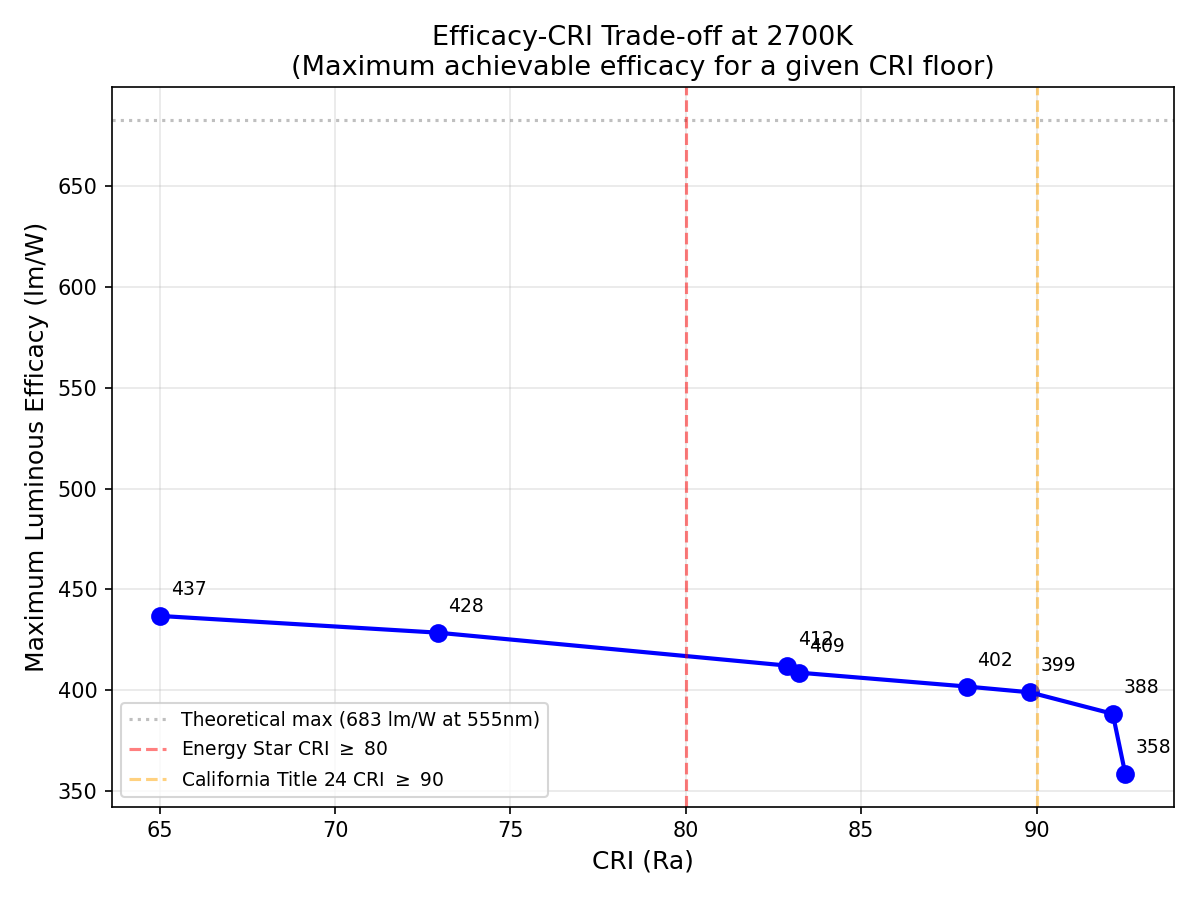
\includegraphics[width=0.75\textwidth]{fig5_tradeoff.png}
\caption{Pareto frontier: maximum luminous efficacy vs.\ minimum CRI at
  2700K.  Vertical dashed lines show the Energy Star (CRI~$\geq$~80) and
  California Title~24 (CRI~$\geq$~90) thresholds.  The theoretical maximum
  at 555~nm is 683~lm/W.  The curve shows rapidly diminishing returns:
  moving from CRI~82 to CRI~98 costs about 80~lm/W.}
\label{fig:tradeoff}
\end{figure}

\subsection{$R_9$ vs.\ Efficacy: The Red Rendering Penalty}

Figure~\ref{fig:r9-vs-eff} shows the key result: at the EU minimum
CRI~$\geq$~80, the optimal spectrum achieves 412~lm/W theoretical
luminous efficacy of radiation (LER) but with $R_9 = 21$.  Saturated reds
are rendered at only one-fifth of their reference fidelity.  To achieve
California JA8's $R_9 \geq 50$ requirement, CRI must be pushed above 90,
reducing achievable efficacy to $\sim$399~lm/W.

\begin{figure}[H]
\centering
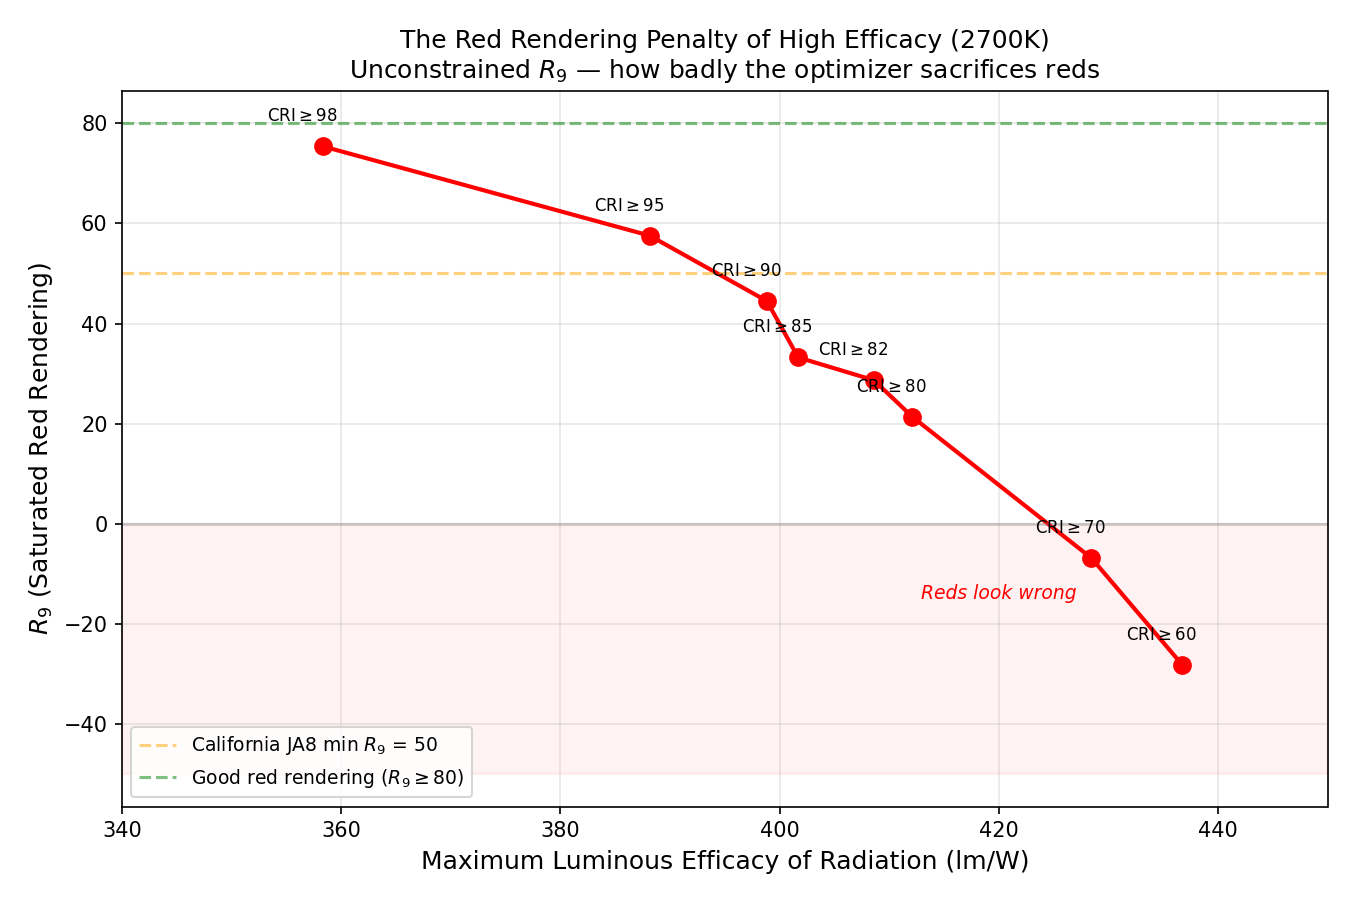
\includegraphics[width=0.80\textwidth]{fig6_r9_vs_efficacy.png}
\caption{$R_9$ (saturated red rendering index) as a function of
  maximum achievable luminous efficacy of radiation at 2700K.
  Each point represents the optimal spectrum at a different CRI floor,
  with $R_9$ unconstrained.  At the EU minimum (CRI~$\geq$~80), $R_9$
  is only 21.  The California JA8 minimum of $R_9 \geq 50$ is not met
  until CRI~$\geq$~90.}
\label{fig:r9-vs-eff}
\end{figure}

These are theoretical radiation-only efficacies assuming unit quantum
efficiency.  For real phosphor-converted LED lamps, Koedam and Opstelten
estimated a $\sim$20\% reduction due to realistic quantum efficiency and
Stokes losses~\cite{walter1978}.  The correction is wavelength-dependent:
converting a 450~nm blue pump photon to a longer-wavelength visible photon
loses a fraction $1 - 450/\lambda_{\text{em}}$ of the photon energy as heat
(the Stokes shift).  Table~\ref{tab:stokes} shows the penalty for
representative LED phosphors.

\begin{table}[H]
\centering
\caption{Stokes loss and quantum yield for LED phosphors
  (450~nm blue pump).}
\label{tab:stokes}
\begin{tabular}{llcccc}
\toprule
Phosphor & Emission & $\lambda_{\text{em}}$ & Stokes & Typ.\ QY & Net \\
         & color    & (nm)                   & loss   &          & loss \\
\midrule
YAG:Ce           & yellow & 560 & 19.6\% & 96\% & 23\% \\
$\beta$-SiAlON:Eu & green  & 535 & 15.9\% & 83\% & 30\% \\
KSF (K$_2$SiF$_6$:Mn) & red & 631 & 28.7\% & 95\% & 33\% \\
Nitride (CASN)   & deep red & 650 & 30.8\% & 88\% & 39\% \\
\bottomrule
\end{tabular}
\end{table}

Adding red phosphor content --- needed for good $R_9$ --- incurs a
\emph{double} penalty: (1)~the Stokes loss is higher (29--31\% vs.\ 16--20\%
for green/yellow), and (2)~the eye's photopic sensitivity $V(\lambda)$ drops
steeply in the red, so each red photon contributes fewer lumens.
This is exactly why the optimizer suppresses red emission when $R_9$
is unconstrained, and why achieving good red rendering in real LED lamps
is expensive in terms of system efficacy.

\section{Discussion}

\subsection{The Regulatory Paradox}

The results reveal a paradox in lighting regulation:

\begin{enumerate}
\item Regulations set a \emph{minimum CRI} (typically 80) and a
      \emph{minimum efficacy} (80--100~lm/W and rising).
\item The optimal solution for high efficacy at moderate CRI is a
      narrow-band, spiky spectrum.
\item Spiky spectra can achieve high CRI scores (by construction ---
      the 8 test colors are rendered well) while having poor real-world
      color rendering (especially saturated colors, TCS~9--14).
\item As efficacy requirements increase over time, manufacturers are
      pushed further toward spiky spectra.
\item The ``efficient'' lamp of the future satisfies all regulations
      but produces light that looks \emph{wrong} to many observers.
\end{enumerate}

This is not a hypothetical concern.  Commercial tri-phosphor fluorescent
lamps and phosphor-converted LEDs already exploit exactly this trade-off.
Their spectral power distributions, with 3--5 peaks and deep valleys, are
the market's practical approximation to the mathematically optimal solution
computed here.

Table~\ref{tab:regulations} compares the major regulatory frameworks.
The EU sets CRI~$\geq$~80 with no $R_9$ requirement; our optimizer
shows that this permits $R_9 = 21$ (Table~\ref{tab:tradeoff}).  The US
DOE 2028 standard requires $\sim$125~lm/W system efficacy but imposes no
color quality floor at all.  Only California JA8 mandates $R_9 \geq 50$
together with CRI~$\geq$~90.

\begin{table}[H]
\centering
\caption{Regulatory landscape for general-service lamps (2025--2026).}
\label{tab:regulations}
\begin{tabular}{lcccc}
\toprule
& EU 2019/2020 & US DOE 2022 & US DOE 2028 & CA Title~24 JA8 \\
\midrule
Min system efficacy$^*$ & $\sim$98 & 45 & 125 & 45 \\
Min CRI ($R_a$)         & 80 & --- & --- & 90 \\
Min $R_9$               & --- & --- & --- & 50 \\
CCT range               & any & any & any & 2700--4000~K \\
\bottomrule
\multicolumn{5}{l}{\small $^*$lm/W for an 800~lm non-directional lamp.}
\end{tabular}
\end{table}

\subsection{Comparison with Thornton's Work}

Thornton arrived at his prime-color wavelengths (450, 540, 610~nm) through
a combination of psychophysical experiments and engineering intuition in the
1970s~\cite{thornton1971,thornton1972cdi,thornton1972three}.  The
\texttt{photopic} optimizer, starting from first principles (Planck's law,
CIE color matching functions, von~Kries adaptation), converges to the same
wavelengths.  This provides independent numerical confirmation of Thornton's
insight.

The deeper significance is that the prime-color wavelengths are not arbitrary
--- they are the eigenvectors of the human visual system's color discrimination
capacity, weighted by luminous sensitivity.

\subsection{What the Regulations Should Do}

The IES TM-30-15 standard addresses some of these problems by using 99 test
color samples instead of 8, and reporting both \emph{fidelity} and
\emph{gamut area}.  Mandating minimum $R_9$ scores (as some California
specifications do) partially closes the red-rendering loophole.  But the
fundamental tension between efficacy and color quality is a physical
constraint that no regulation can eliminate --- it can only choose where
on the Pareto frontier to operate.

\section{Literature Review}

The optimization of white-light spectra has a history reaching back to
the 1950s, but two papers from the 1970s are particularly relevant to the
present work: Thornton's 1971 study of prime colors and Walter's 1978
application of nonlinear programming to lamp spectra.

\subsection{Thornton (1971): Prime Colors and the Structure of White Light}

W.~A.~Thornton of Westinghouse~\cite{thornton1971} posed the question:
\emph{What is the optimum spectral power distribution of artificial white
light?}  Starting from the CIE luminosity function $\bar{y}(\lambda)$ and the
IES--CIE color rendering index, Thornton evaluated white light composed
of three spectral lines.  By systematic variation of each wavelength while
holding the other two fixed (at 450, 540, and 610~nm), he showed that
these three wavelengths are local optima of both CRI and a combined
figure of merit $\text{FM} = 320\eta + \text{CRI}$.

Thornton's key findings:
\begin{itemize}
\item Three spectral lines at \textbf{450, 540, and 610~nm} --- the
  ``prime colors'' --- yield white light superior to commercial
  fluorescent lamps of the same chromaticity in \emph{both} luminosity and
  CRI.  Three-line light at 4200~K achieved $\eta = 0.58$, CRI~$=$~71,
  compared to $\eta = 0.48$, CRI~$=$~67 for a commercial cool-white
  fluorescent.
\item Wavelengths near \textbf{495 and 575~nm} are ``anti-prime'':
  they degrade CRI without contributing significantly to luminosity.
  Removing a slice of power near 500 or 580~nm from a cool-white
  lamp's spectrum actually \emph{raises} the CRI.
\item A 1966 demonstration with interference filters and projectors showed
  that 60 observers judged three-line prime-color light as providing
  ``very good, if not excellent'' color rendering of meat, vegetables,
  flowers, and skin tones.
\item The prime-color wavelengths correspond to the maxima of
  \emph{tristimulus difference functions}
  $\bar{b} = \bar{z} - \bar{x} - \bar{y}$,
  $\bar{g} = \bar{y} - \bar{x} - \bar{z}$,
  $\bar{r} = \bar{x} - \bar{y} - \bar{z}$,
  which Thornton termed ``bluminosity,'' ``verdinosity,'' and ``rubinosity.''
  He proposed corresponding units (blumen, verden, ruben) analogous to the
  lumen, and showed that rubinosity $\rho$ is an excellent predictor of red
  phosphor performance in tri-phosphor blends (Fig.~14 in the original).
\end{itemize}

Thornton's insight is that the prime-color wavelengths are not arbitrary
engineering choices but reflect the structure of human color vision: they
are the wavelengths that ``pull hardest'' toward their chromaticities per
watt of power, and are therefore the most efficient at establishing a
wide color gamut from a small number of spectral components.

\subsection{Walter (1978): Nonlinear Programming of Lamp Spectra}

Wolfgang Walter of GTE Sylvania~\cite{walter1978} took a fundamentally
different approach: rather than assuming a fixed number of spectral bands
and optimizing their positions, he applied \emph{nonlinear mathematical
programming} (the generalized reduced gradient algorithm of Lasdon et
al.)\ to find optimal spectra with \emph{no a priori constraint on shape}.
The spectrum was discretized into 31 variables (10~nm intervals from
400--700~nm), with the objective of maximizing luminous flux of a
40-watt fluorescent lamp subject to constraints on total UV excitation
power, ANSI chromaticity ellipses, and a CRI floor.

Walter's key results:
\begin{itemize}
\item Optimal spectra with CRI up to 90--95 consist of \textbf{just four
  narrow bands}, positioned at approximately 460, 530, 580, and 620~nm,
  stable across all four ANSI lamp types (cool white, white, warm white,
  daylight).
\item The unconstrained (CRI-free) optimum is a two-line spectrum (the
  MacAdam pair), confirming earlier theoretical work.
\item As CRI constraints increase from 50 to 95, additional bands
  appear and existing bands broaden, with a monotonic decrease in
  luminous efficacy (from $\sim$140~lm/W at CRI~50 to $\sim$107~lm/W at
  CRI~95 for cool white).
\item The optimization surface is ``fairly flat'' near the optimum:
  small perturbations to the SPD do not greatly affect luminance or CRI,
  suggesting practical tolerance for real phosphor emission profiles.
\item When \emph{all} component indices $R_j \geq C$ are required (not just
  the average $R_a$), efficacy drops further --- confirming that the CRI
  average conceals weaknesses in individual color samples.
\end{itemize}

The published discussion section is notable: Koedam and Opstelten of
Philips argued that the four-band optimum offers ``no real improvement''
over the Philips three-band lamp after correcting for realistic quantum
efficiency ($\sim$80\% rather than 100\%).  Thornton himself commented,
noting that if subjective criteria (color preference, visual clarity,
perceived brightness) are considered rather than CRI alone, three bands
may be superior to four.

\subsection{Relationship to Our Results}

Our \texttt{photopic} optimizer, approaching the problem from yet another
direction --- continuous piecewise-linear log-amplitude perturbation of a
blackbody, optimized by COBYLA --- independently converges to essentially
the same spectral structure.  The three-peak topology that dominates our
results at low CRI floors (437~lm/W at CRI~$\geq$~60) corresponds to
Thornton's prime colors, while the broadening and addition of a fourth
peak at higher CRI floors (CRI~$\geq$~90 and above) matches Walter's
four-band result.  The wavelength positions we find ($\sim$450, $\sim$540,
$\sim$610~nm) agree with Thornton to within the resolution of our spectral
parameterization.

The consistency across three independent methods --- Thornton's
parametric three-line analysis, Walter's unconstrained nonlinear
programming, and our hierarchical COBYLA optimization --- provides strong
evidence that the prime-color structure is a genuine feature of the
CRI/efficacy optimization landscape, not an artifact of any particular
numerical method.

\section{The Deficiencies of CRI and the Legislative Paradox}

\subsection{Why CRI is Known to be Wrong}

The CIE Color Rendering Index (CRI, $R_a$) has been recognized as
flawed since at least the 1980s, yet it remains the dominant regulatory
metric.  The principal deficiencies are:

\begin{enumerate}
\item \textbf{Only 8 unsaturated test samples.}  $R_a$ averages $R_1$
  through $R_8$, all of which are low-chroma, pastel-like Munsell
  samples.  Saturated colors --- which are the ones most affected by
  narrow-band spectra --- are represented only in $R_9$--$R_{14}$, which
  are reported but \emph{not} included in the official score.  This is the
  loophole our optimizer exploits: it can drive $R_9$ (saturated red) to
  $-28$ while maintaining $R_a = 65$.

\item \textbf{Von Kries adaptation model.}  The CRI uses a simple
  diagonal (von Kries) chromatic adaptation transform, which is known to
  be a poor approximation of human color constancy, especially for
  narrow-band illuminants far from the blackbody locus.

\item \textbf{Uniform color space.}  The CRI computes color shifts in the
  CIE~1964 $U^*V^*W^*$ space, which is perceptually nonuniform.
  Equal $\Delta E$ values do not correspond to equal perceived color
  differences.

\item \textbf{Averaging hides problems.}  A lamp with seven $R_i = 95$
  and one $R_i = 25$ gets $R_a = 86$ --- an apparently acceptable score
  that conceals a severe deficiency in one color region.  Walter's work
  showed that requiring all $R_j \geq C$ rather than just $R_a \geq C$
  significantly changes the optimal spectrum and reduces achievable
  efficacy.

\item \textbf{Penalizes increased saturation.}  Because CRI measures
  \emph{fidelity} (closeness to the reference illuminant), a lamp that
  renders colors \emph{more} saturated than the reference --- which
  people often prefer --- receives a \emph{lower} CRI score.
  Thornton's color preference index (CPI) and the IES TM-30-15
  standard~\cite{tm30} address this.
\end{enumerate}

\subsection{Why Legislators Use It Anyway}

Despite these well-known deficiencies, CRI remains the basis for
lighting regulations worldwide (EU Ecodesign 2019/2020, US DOE/EISA,
California Title~24, Energy Star).  The reasons are partly institutional
inertia and partly the absence of a universally agreed replacement:

\begin{itemize}
\item \textbf{IES TM-30-15/18} defines two metrics: $R_f$ (fidelity,
  similar to CRI but with 99 test samples and CAM02-UCS) and $R_g$ (gamut
  area, measuring saturation changes).  It is technically superior but
  has not yet been mandated by any major regulatory body.
\item \textbf{CIE~224:2017} proposed a general color fidelity index $R_f$
  similar to TM-30, but adoption has been slow.
\item The lighting industry has decades of CRI-referenced product data,
  specifications, and marketing materials.  Changing the metric would
  require re-characterizing the entire installed base.
\end{itemize}

The result is a regulatory landscape that \emph{incentivizes} the very
spiky, CRI-gaming spectra that our optimizer finds.  Manufacturers who
maximize efficacy while just meeting CRI~$\geq$~80 are rewarded by the
regulatory framework, even though the resulting light may render saturated
colors poorly.  The ``weird final state'' is not a theoretical curiosity
--- it is the market equilibrium toward which regulations push.

\section{Future Work}

Several directions suggest themselves:

\begin{enumerate}
\item \textbf{$R_9$ as a function of required efficacy.}  The most
  practically important question is: under a given regulatory framework
  (e.g., EU Ecodesign minimum efficacy), what is the \emph{achievable}
  $R_9$ (saturated red rendering)?  Our current runs fix the CRI floor
  and let efficacy be the objective.  The dual problem --- fix efficacy
  and maximize $R_9$ --- would map out the ``quality frontier'' that
  regulations actually define.  Similarly, sweeping over required
  efficacy at fixed CRI floor would show how $R_9$ degrades as efficiency
  pressure increases.

\item \textbf{Realistic quantum efficiency.}  Our calculations assume
  unit quantum efficiency, following Walter's approach.  Real
  phosphors have wavelength-dependent quantum efficiencies $\eta_Q(\lambda)$,
  typically 80--95\% for blue/green and dropping for deep red.
  Koedam and Opstelten noted that applying realistic $\eta_Q$ reduces
  calculated efficacy by $\sim$20\%.  Incorporating $\eta_Q(\lambda)$
  into the objective function would shift the optimal peak positions
  and show whether the three-peak structure survives under real-world
  conversion losses.

\item \textbf{TM-30 optimization.}  Replace the CRI constraint with
  TM-30 $R_f$ and $R_g$ metrics.  Because TM-30 uses 99 test samples and
  a more uniform color space, the optimizer would have far less room to
  exploit loopholes.  The resulting spectra may be broader and more
  natural-looking.

\item \textbf{Multiple CCTs.}  Extend the analysis to the full range of
  commercial color temperatures (2700--6500~K).  Walter showed that the
  four-band positions are remarkably stable across ANSI lamp types;
  verifying this with our continuous parameterization would be valuable.

\item \textbf{LED-realistic spectra.}  Constrain the spectrum to
  physically realizable LED spectra: a narrow blue pump peak
  ($\sim$450~nm, 20~nm FWHM) plus one or more phosphor emission bands
  (50--100~nm FWHM, constrained shapes).  This would bridge the gap
  between our theoretical optima and practical LED design.

\item \textbf{Scotopic/mesopic efficacy.}  Outdoor and roadway lighting
  operates at mesopic light levels where the scotopic sensitivity
  function $V'(\lambda)$ contributes.  The S/P ratio (scotopic to photopic
  luminance ratio) is an additional design variable that regulations are
  beginning to address.

\item \textbf{Circadian impact.}  Blue-rich spectra suppress melatonin
  production.  A constraint on melanopic equivalent daylight illuminance
  (M-EDI) could be added to the optimization, capturing the tension
  between visual efficacy and biological impact.
\end{enumerate}

\section{Conclusion}

The constrained optimization of light spectra reveals that regulatory
pressure on luminous efficacy drives lamp spectra toward a mathematically
determined ``weird'' final state: three narrow spectral peaks near 450,
540, and 610~nm with suppressed emission elsewhere.  This state maximizes
lumens per watt while technically satisfying color rendering requirements,
but at the cost of poor rendering of saturated colors --- especially reds.

The \texttt{photopic} tool, built as a hybrid Modula-3/Scheme application,
enables rapid exploration of this trade-off space using COBYLA constrained
optimization with hierarchical spectral resolution.

\section*{Availability}

The \texttt{photopic} tool, this report, the optimization data, and all
plotting scripts are open source.  The source code is available in two
repositories:

\begin{itemize}
\item \textbf{Photopic tool and data:}
  \url{https://github.com/IntelLabs/async-toolkit}, branch
  \texttt{claude\_edits}, path
  \texttt{m3utils/m3utils/photopic/}.
  The report and optimization results are in
  \texttt{photopic/report-runs/}.

\item \textbf{CM3 compiler, MScheme, and runtime libraries:}
  \url{https://github.com/modula3/cm3}.
  MScheme lives in \texttt{m3-scheme/}; the COBYLA binding, spectral
  libraries, and CIE data are in the \texttt{m3utils} tree above.
\end{itemize}

\noindent
Both repositories are licensed under open-source terms (Apache~2.0 for
the async-toolkit; BSD for CM3).

\begin{thebibliography}{99}

\bibitem{thornton1971}
W.~A.~Thornton,
``Luminosity and color-rendering capability of white light,''
\emph{J. Opt. Soc. Am.}, vol.~61, no.~9, pp.~1155--1163, 1971.

\bibitem{thornton1972cdi}
W.~A.~Thornton,
``Color-discrimination index,''
\emph{J. Opt. Soc. Am.}, vol.~62, no.~2, pp.~191--194, 1972.

\bibitem{thornton1972three}
W.~A.~Thornton,
``Three-color visual response,''
\emph{J. Opt. Soc. Am.}, vol.~62, no.~3, pp.~457--459, 1972.

\bibitem{thornton-inventor}
``Prime Color, Inc.\ --- Founder,'' \url{http://www.prime-color.com/founder.htm}.
W.~A.~Thornton received the 1979 U.S. National Inventor of the Year award
for his prime-color electro-luminescence patents.

\bibitem{foley-vandam}
J.~D.~Foley, A.~van~Dam, S.~K.~Feiner, and J.~F.~Hughes,
\emph{Computer Graphics: Principles and Practice}, 2nd~ed.
Addison-Wesley, 1990. (CIE colorimetric formulas.)

\bibitem{powell1994}
M.~J.~D.~Powell,
``A direct search optimization method that models the objective and
constraint functions by linear interpolation,''
in \emph{Advances in Optimization and Numerical Analysis},
S.~Gomez and J.-P.~Hennart, Eds. Kluwer, 1994, pp.~51--67.

\bibitem{hung-tsao2013}
P.-C.~Hung and J.~Y.~Tsao,
``Maximum white luminous efficacy of radiation versus color rendering index
and color temperature: exact results and a useful analytic expression,''
\emph{J. Display Technology}, vol.~9, no.~6, pp.~405--412, 2013.

\bibitem{murphy2012}
T.~W.~Murphy~Jr.,
``Maximum spectral luminous efficacy of white light,''
\emph{J. Appl. Phys.}, vol.~111, 104909, 2012.

\bibitem{ohno2004}
Y.~Ohno,
``Color rendering and luminous efficacy of white LED spectra,''
\emph{Proc.\ SPIE}, vol.~5530, 2004.

\bibitem{walter1978}
W.~Walter,
``Optimum lamp spectra,''
\emph{J.\ Illuminating Engineering Society}, vol.~7, no.~2, pp.~66--73,
1978.

\bibitem{modula3}
L.~Cardelli, J.~Donahue, L.~Glassman, M.~Jordan, B.~Kalsow, and
G.~Nelson,
``Modula-3 language definition,''
\emph{ACM SIGPLAN Notices}, vol.~27, no.~8, pp.~15--42, 1992.

\bibitem{cm3}
Critical Mass Modula-3 (CM3),
\url{https://github.com/modula3/cm3}, 2024.

\bibitem{mscheme}
MScheme: A Scheme interpreter embedded in Modula-3,
in the CM3 distribution, \texttt{m3-scheme/} package.

\bibitem{tm30}
IES~TM-30-18,
``IES method for evaluating light source color rendition,''
Illuminating Engineering Society, New York, 2018.

\end{thebibliography}

\end{document}
